 %package list
\documentclass{article}
\usepackage[top=3cm, bottom=3cm, outer=3cm, inner=3cm]{geometry}
\usepackage{multicol}
\UseRawInputEncoding
\usepackage{graphicx}
\usepackage{url}
%\usepackage{cite}
\usepackage{hyperref}
\usepackage{array}
%\usepackage{multicol}
\newcolumntype{x}[1]{>{\centering\arraybackslash\hspace{0pt}}p{#1}}
\usepackage{natbib}
\usepackage{pdfpages}
\usepackage{multirow}
\usepackage[normalem]{ulem}
\useunder{\uline}{\ul}{}
\usepackage{svg}
\usepackage{xcolor}
\usepackage{listings}
\lstdefinestyle{ascii-tree}{
    literate={├}{|}1 {─}{--}1 {└}{+}1
  }
\lstset{basicstyle=\ttfamily,
  showstringspaces=false,
  commentstyle=\color{red},
  keywordstyle=\color{blue}
}
%\usepackage{booktabs}
\usepackage{caption}
\usepackage{subcaption}
\usepackage{float}
\usepackage{array}

\newcolumntype{M}[1]{>{\centering\arraybackslash}m{#1}}
\newcolumntype{N}{@{}m{0pt}@{}}

%------------------------------ ÍTEMS -------------------------------

\newcommand{\itemEmail}{hchoquehuancaz@unsa.edu.pe}
\newcommand{\itemStudent}{Hernan Andy Choquehuanca Zapana}
\newcommand{\itemCourse}{Fundamentos de la Programacion II}
\newcommand{\itemCourseCode}{20232191}
\newcommand{\itemSemester}{II}
\newcommand{\itemUniversity}{Universidad Nacional de San Agustin de Arequipa}
\newcommand{\itemFaculty}{Facultad de Ingenieria de Produccion y Servicios}
\newcommand{\itemDepartment}{Departamento Academico de Ingenieria de Sistemas e Informatica}
\newcommand{\itemSchool}{Escuela Profesional de Ingenieria de Sistemas}
\newcommand{\itemAcademic}{2023 - B}
\newcommand{\itemInput}{Del 18 Octubre 2023}
\newcommand{\itemOutput}{Al 23 Octubre 2023}
\newcommand{\itemPracticeNumber}{07}
\newcommand{\itemTheme}{Combinando Arreglos Estandar y ArrayList}

%------------------------------  ------------------------------

\usepackage[english,spanish]{babel}
\usepackage[utf8]{inputenc}
\AtBeginDocument{\selectlanguage{Spanish}}
\renewcommand{\figurename}{Figura}
\renewcommand{\refname}{Referencias}
\renewcommand{\tablename}{Tabla} %esto no funciona cuando se usa babel
\AtBeginDocument{
	\renewcommand\tablename{Tabla}
}

\usepackage{fancyhdr}
\pagestyle{fancy}
\fancyhf{}
\setlength{\headheight}{30pt}
\renewcommand{\headrulewidth}{1pt}
\renewcommand{\footrulewidth}{1pt}
\fancyhead[L]{\raisebox{-0.2\height}{
\includegraphics[width=3cm]{img/logo_episunsa.png}}}
\fancyhead[C]{\fontsize{7}{7}\selectfont	\itemUniversity \\ \itemFaculty \\ \itemDepartment \\ \itemSchool \\ \textbf{\itemCourse}}
\fancyhead[R]{\raisebox{-0.2\height}{
\includegraphics[width=1.2cm]{img/logo_abet}}}
\fancyfoot[L]{Estudiante: Hernan Choquehuanca Zapana}
\fancyfoot[R]{\itemCourse}
\fancyfoot[C]{Página \thepage}

% para el codigo fuente
\usepackage{listings}
\usepackage{color, colortbl}
\definecolor{dkgreen}{rgb}{0,0.6,0}
\definecolor{gray}{rgb}{0.5,0.5,0.5}
\definecolor{mauve}{rgb}{0.58,0,0.82}
\definecolor{codebackground}{rgb}{0.95, 0.95, 0.92}
\definecolor{tablebackground}{rgb}{0.8, 0, 0}

\lstset{frame=tb,
	language=bash,
	aboveskip=3mm,
	belowskip=3mm,
	showstringspaces=false,
	columns=flexible,
	basicstyle={\small\ttfamily},
	numbers=none,
	numberstyle=\tiny\color{gray},
	keywordstyle=\color{blue},
	commentstyle=\color{dkgreen},
	stringstyle=\color{mauve},
	breaklines=true,
	breakatwhitespace=true,
	tabsize=3,
	backgroundcolor= \color{codebackground},
}

%------------------------------ INICIO DEL DOCUMENTO------------------------------

\begin{document}
	
	\vspace*{10px}
	
	\begin{center}	
		\fontsize{17}{17} \textbf{ Informe de Laboratorio \itemPracticeNumber}
	\end{center}
	\centerline{\textbf{\Large Tema: \itemTheme}}
	%\vspace*{0.5cm}	

	\begin{flushright}
		\begin{tabular}{|M{2.5cm}|N|}
			\hline 
			\rowcolor{tablebackground}
			\color{white} \textbf{Nota}  \\
			\hline 
			     \\[30pt]
			\hline 			
		\end{tabular}
	\end{flushright}	

	\begin{table}[H]
		\begin{tabular}{|x{4.7cm}|x{4.8cm}|x{4.8cm}|}
			\hline 
			\rowcolor{tablebackground}
			\color{white} \textbf{Estudiante} & \color{white}\textbf{Escuela}  & \color{white}\textbf{Asignatura}   \\
			\hline 
			{\itemStudent \par \itemEmail} & \itemSchool & {\itemCourse \par Semestre: \itemSemester \par Código: \itemCourseCode}     \\
			\hline 			
		\end{tabular}
	\end{table}		
	
	\begin{table}[H]
		\begin{tabular}{|x{4.7cm}|x{4.8cm}|x{4.8cm}|}
			\hline 
			\rowcolor{tablebackground}
			\color{white}\textbf{Laboratorio} & \color{white}\textbf{Tema}  & \color{white}\textbf{Duración}   \\
			\hline 
			\itemPracticeNumber & \itemTheme & 02 horas   \\
			\hline 
		\end{tabular}
	\end{table}
	
	\begin{table}[H]
		\begin{tabular}{|x{4.7cm}|x{4.8cm}|x{4.8cm}|}
			\hline 
			\rowcolor{tablebackground}
			\color{white}\textbf{Semestre académico} & \color{white}\textbf{Fecha de inicio}  & \color{white}\textbf{Fecha de entrega}   \\
			\hline 
			\itemAcademic & \itemInput &  \itemOutput  \\
			\hline 
		\end{tabular}
	\end{table}


%------------------------------ ACTIVIDADES (TAREA) ------------------------------

	\section{Tarea}
	\begin{itemize}		
        \item Cree un Proyecto llamado Laboratorio7
        \item Usted deberá crear las dos clases Soldado.java y VideoJuego4.java. Puede reutilizar lo
        desarrollado en Laboratorios anteriores.
        \item Del Soldado nos importa el nombre, puntos de vida, fila y columna (posición en el tablero).
        \item El juego se desarrollará en el mismo tablero de los laboratorios anteriores. Para el tablero
        utilizar la estructura de datos más adecuada.
        \item Tendrá 2 Ejércitos (utilizar la estructura de datos más adecuada). Inicializar el tablero con n
        soldados aleatorios entre 1 y 10 para cada Ejército. Cada soldado tendrá un nombre
        autogenerado: Soldado0X1, Soldado1X1, etc., un valor de puntos de vida autogenerado
        aleatoriamente [1..5], la fila y columna también autogenerados aleatoriamente (no puede
        haber 2 soldados en el mismo cuadrado). Se debe mostrar el tablero con todos los soldados
        creados y sus puntos de vida. Además de los datos del Soldado con mayor vida de cada ejército, el
        promedio de puntos de vida de todos los soldados creados por ejército, los datos de todos los
        soldados por ejército en el orden que fueron creados y un ranking de poder de todos los
        soldados creados por ejército (del que tiene más nivel de vida al que tiene menos) usando 2 diferentes algoritmos de ordenamiento. Finalmente, que muestre qué ejército ganará la batalla (indicar la métrica usada para decidir al ganador de la batalla). Hacer el programa iterativo.

	\end{itemize}
		
	\section{Equipos, materiales y temas utilizados}
	\begin{itemize}
		\item Sistema Operativo Windows 11 Pro 22H2 64 bits.
		\item Visual Studio Code.
		\item Git 2.42.0.
		\item Cuenta en GitHub con el correo institucional.
        \item Editor LaTeX en línea Overleaf.
        \item Variables Simples
        \item Métodos.
        \item Métodos de Búsqueda y Ordenamiento.
        \item Arreglos Estándar y Bidimensionales.
        \item ArrayList
        
        
	\end{itemize}
	
	\section{URL de Repositorio Github}
	\begin{itemize}
		\item URL del Repositorio GitHub para clonar o recuperar.
        \item \url{https://github.com/hernanchoquehuanca/fp2-23b.git}
		\item URL para el laboratorio 07 en el Repositorio GitHub.
		\item \url{https://github.com/hernanchoquehuanca/fp2-23b/tree/main/fase02/lab07}
	\end{itemize}
	
	\section{Trabajo del Laboratorio 07}
        
        
%-----------------------------------------------------------------------------------
%------------------------------------- ACTIVIDADES  --------------------------------
%-----------------------------------------------------------------------------------

% ACTIVIDADESSSS

    \subsection{Actividad 01}
    
        \subsubsection{Clase Soldado.java}
        \begin{itemize}	
            \item Haciendo uso de la clase Soldado.java del laboratorio anterior (lab06), se adaptó al ejercicio actual.
            \begin{itemize}
                \item Primero copiamos el código tal cual a la carpeta del laboratorio actual (lab07).
            \end{itemize}
        \end{itemize}

        \begin{lstlisting}[language=bash,caption={Commit \href{https://github.com/hernanchoquehuanca/fp2-23b/commit/88096212a7228ae8637f2b46b77eee9abe96f443}{8809621}: En el primer commit se reutilizaba la clase Soldado.java del laboratorio anterior (lab06)}][H]
    		$ git add .
    		$ git commit -m "Reutilizando las clases Soldado.java y VideoJuego3.java del Lab06"
    		$ git push -u origin main
    	\end{lstlisting}
        \newpage
        \begin{itemize}
            \item Nuestra clase Soldado tendrá los siguientes atributos:
            \begin{itemize}
                \item name (Nombre).
                \item row (Fila).
                \item column (Columna).
                \item status (Estado).
                \item health (Vida).
                \item team (Equipo).
            \end{itemize}
            
        \end{itemize}
        \lstinputlisting[language=Java, firstline=2, lastline=7, firstnumber=2,numbers=left,]{src/Soldado.java}

        \begin{itemize}
            \item Además creamos el método constructor, tendiendo en cuenta que tiene que tener el mismo nombre que la clase y considerando sus atributos como parámetros:
            \begin{itemize}
                \item Se utilizó el puntero \textcolor{blue}{this} para evitar ambigüedades.
            \end{itemize}
        \end{itemize}

        \lstinputlisting[language=Java, firstline=9, lastline=16, firstnumber=9,numbers=left,]{src/Soldado.java}

        \begin{itemize}
            \item Luego de ello también se implementaron los getters y setters para cada atributo de nuestra clase Soldado.
            \begin{itemize}
                \item Setters: 
            \end{itemize}
        \end{itemize}

        \lstinputlisting[language=Java, firstline=18, lastline=35,firstnumber=18,numbers=left]{src/Soldado.java}

        \begin{itemize}
            \begin{itemize}
                \item Getters: 
            \end{itemize}
        \end{itemize}

        \lstinputlisting[language=Java, firstline=37, lastline=54,firstnumber=37,numbers=left]{src/Soldado.java}

        \begin{lstlisting}[language=bash,caption={Commit \href{https://github.com/hernanchoquehuanca/fp2-23b/commit/a43020e7ffdcd7aca45a9bd5bcc58bf90ce02059}{a43020e} - \href{https://github.com/hernanchoquehuanca/fp2-23b/commit/598a62d5d65db6832192e50b6ef383709a550043}{61b7b8e}: Se concluía la clase Soldado.java agregando su atributo team, que en el lab06 no se tomaba en cuentat}][H]
    		$ git add .
    		$ git commit -m "Agregando el atributo team a la clase Soldado.java, esto servira para usarlo al momento de mostrar la tabla y sea mas funcional, ademas se adapto el codigo para trabajar con este atributo"			
    		$ git push -u origin main
    	\end{lstlisting
        \end{lstlisting}

        \begin{itemize}
            \item Y finalizando con esta clase, se creo el método toString().
            \begin{itemize}
                \item Se agregó la anotación \textcolor{blue}{@Override} para indicar que se está reemplazando el método de su clase padre \textcolor{blue}{Objetct}.
                \item En este método se considera los atributos de la clase (name, row, column, status, health, team).
                \item Se utilizaron saltos de con ayuda del \textcolor{blue}{\textbackslash n}.
            \end{itemize}
        \end{itemize}

        \lstinputlisting[language=Java, firstline=55, lastline=64,firstnumber=55,numbers=left]{src/Soldado.java}
\newpage
        \begin{itemize}
            \begin{itemize}
                \item Un ejemplo de como se muestra en la siguiente imagen:
            \end{itemize}
        \end{itemize}
            
        \begin{figure}[H]
            \centering
            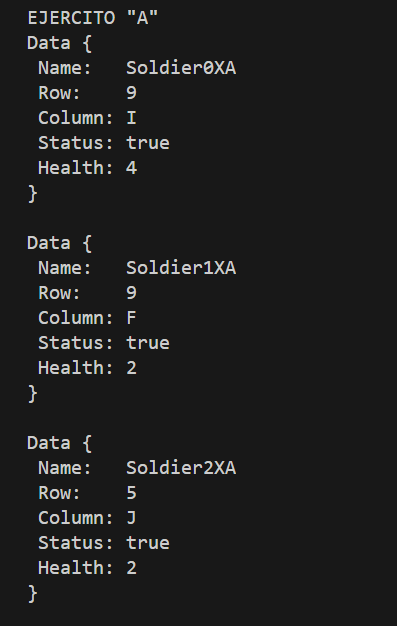
\includegraphics[width=0.42\textwidth,keepaspectratio]{img/toString.png}
            \caption{}
        \end{figure}
     
        %%%%%%%%%%%%%%%%
        
        \subsubsection{Clase VideoJuego.java}

        \begin{itemize}
            \item Primero se comenzó con la creación de la clase. 
            \item Posterior a ello se crearon dos variables de clase: 
            \begin{itemize}
                \item Un ArrayList bidimensional, el cual contendrá a los soldados del ejército.
                \item Además de un ArrayList unidimensional que nos servirá para contener a los soldados creados previamente, de esta manera será más fácil trabajar con ellos en los futuros métodos.
            \end{itemize}
        \end{itemize}

        \lstinputlisting[language=Java, firstline=8, lastline=11,firstnumber=8,numbers=left]{src/VideoJuego4.java}

        \begin{lstlisting}[language=bash,caption={Commit \href{https://github.com/hernanchoquehuanca/fp2-23b/commit/a43020e7ffdcd7aca45a9bd5bcc58bf90ce02059}{a43020e} - \href{https://github.com/hernanchoquehuanca/fp2-23b/commit/a9e7076e698a58a62ad7f89cd6c64a6f778b95e7}{a9e7076}: En el segundo commit se modificaba las variables de la clase VideoJuego4.java para utilizar las más adecuadas, luego más adelante se optó por utilizar ArrayList}][H]
    		$ git add .
    		$ git commit -m "Cambiando la estructura de datos para el tablero, se utilizara un arreglo bidimensional de soldados, el cual sera una variable de la clase VideoJuego4.java"			
    		$ git push -u origin main
    	\end{lstlisting}
     
        %%%%%%%%%%%%%%%%
        \subsubsection{Método para la creación de los ejército}

        \begin{itemize}
            \item El método tiene como nombre \textcolor{blue}{createArmy()}.
            \item Primero se define el número de soldados que contendrá cada ejército, haciendo uso de \textcolor{blue}{Math.random}.
            \item Luego utilizando un doble bucle for, se inicializa el ArrayList bidimensional de soldados en \textcolor{blue}{null}.
            \item Ahora se llama dos veces al método \textcolor{blue}{createArmyTeam} para realizar la creación de los dos ejércitos a partir de los tamaños ya establecidos anteriormente y además el argumento tipo char para el identificador de cada equipo.
        \end{itemize}

        \lstinputlisting[language=Java, firstline=88, lastline=100,firstnumber=88,numbers=left]
        {src/VideoJuego4.java}
        
        \begin{lstlisting}[language=bash,caption={Commit \href{https://github.com/hernanchoquehuanca/fp2-23b/commit/598a62d5d65db6832192e50b6ef383709a550043}{598a62d}: Se implementó el método createArmy()}][H]
    		$ git add .
    		$ git commit -m "Adaptando los metodos createArmy y CreateArmyTeam para que trabajen ahora con los arreglos bidimensionales de soldados que es la estructura de datos de nuestro tablero"			
    		$ git push -u origin main
    	\end{lstlisting}
        
        %%%%%%%%%%%%%%%%
        \subsubsection{Método para la creación de ejércitos}

        \begin{itemize}
            \item El método tiene como nombre \textcolor{blue}{createArmyTeam()}.
            \item Recibe como parámetros un entero que es el número de soldados del ejército, el ArrayList de soldados a utilizar y un String que es el char que va al final del nombre de los soldados, esto último nos ayuda a identificarlos mejor.
            \item Utilizando un do while se crean posiciones aleatorias en el ArrayList bidimensional, tomando como condición que dicha posición sea distinta de \textcolor{blue}{null}.
            \item Finalmente se crea el soldado, se almacena en ambos arreglos y retorna el ArrayList unidimensional con los soldados creados.

        \end{itemize}
        \newpage
        \lstinputlisting[language=Java, firstline=102, lastline=116,firstnumber=102,numbers=left]
        {src/VideoJuego4.java}

        \begin{lstlisting}[language=bash,caption={Commit \href{https://github.com/hernanchoquehuanca/fp2-23b/commit/598a62d5d65db6832192e50b6ef383709a550043}{598a62d} - \href{https://github.com/hernanchoquehuanca/fp2-23b/commit/a9e7076e698a58a62ad7f89cd6c64a6f778b95e7}{a9e7076}: Se modificó el tipo de estructura para el tablero}][H]
    		$ git add .
    		$ git commit -m "Cambiando la estructura de datos del tablero principal, se volvio a utilizar ArrayList de ArrayList de soldados, esto para facilitar que el programa sea iterativo y la opcion de crear nuevos ejercitos sea optima"			
    		$ git push -u origin main
    	\end{lstlisting}
     
        %%%%%%%%%%%%%%%%
        
        \subsubsection{Método para mostrar la tabla con el ejército}

        \begin{itemize}
            \item El método tiene como nombre \textcolor{blue}{showArmyTable()}.
            \item La funcionalidad es simple:
            \begin{itemize}
                \item Se crea el String (\textcolor{blue}{linesDown}), este será usado para la impresión de las lineas inferiores de cada fila de recuadros.
                \item Primeramente se imprime la parte superior, donde se encuentran las letras que indica las columnas. Seguido de una linea que representa la parte superior de la tabla.
                \item Se utilizó un bucle for con dos bucles en su interior, siendo su principal para las filas y los secundarios para las columnas.
                \item En el primero, inicia imprimiendo los datos de los soldados si es que se encuentran, se evalúa si contiene un Soldado o \textcolor{blue}{\texttt{null}}; en caso de ser así, imprimirá \textcolor{violet}{`` |''}, en caso de contener a un soldado completará el cuadrado de la tabla incluyendo ejército (A o B), y su nombre simplificado (S + número generado). 
                \item Dentro del segundo for imprime el número de fila, se agregó una condicional que nos sirve para darle un toque de simetría a esta enumeración de fila, y así evitar que al momento de imprimir el 10 recorra un espacio. Además en caso de que en una posición se encuentre a un soldado, se colocará la vida de este.
                \item Finalmente se imprime linesDown que completaría la línea inferior de cada fila.
            \end{itemize}
        \end{itemize}
\newpage
        \lstinputlisting[language=Java, firstline=118, lastline=137,firstnumber=118,numbers=left]{src/VideoJuego4.java}
        
        \begin{itemize}
            \begin{itemize}
                \item Un ejemplo de como se muestra en la siguiente imagen:
            \end{itemize}
        \end{itemize}

        \begin{figure}[H]
            \centering
            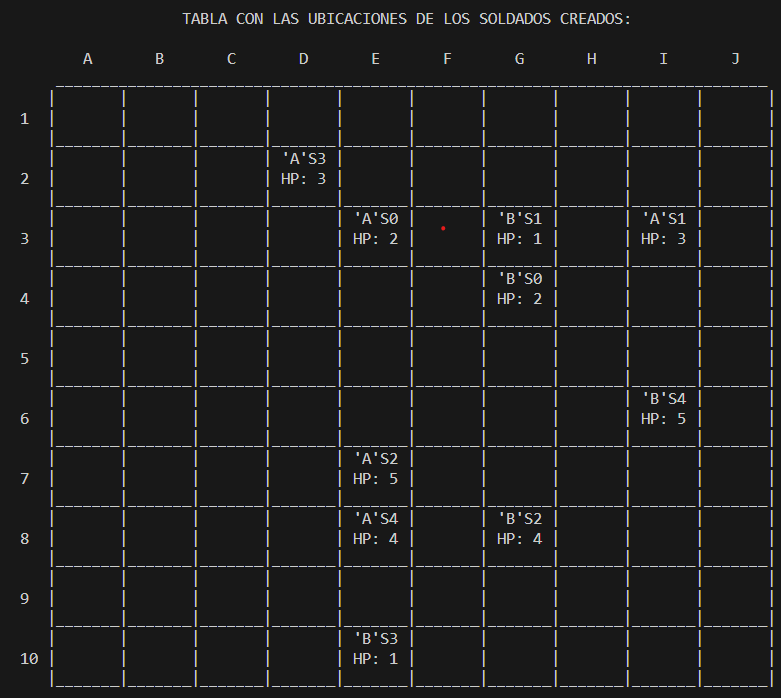
\includegraphics[width=0.65\textwidth,keepaspectratio]{img/showArmyTable.png}
            \caption{}
        \end{figure}

        \begin{lstlisting}[language=bash,caption={Commit \href{https://github.com/hernanchoquehuanca/fp2-23b/commit/4b6ccf86d403513981c5975cadb841d6cd541e61}{4b6ccf8}: Se adaptó e implementó el método para mostrar la tabla con los soldados de ambos ejércitos incluyendo su vida}][H]
    		$ git add .
    		$ git commit -m "Redefiniendo el metodo showTable para que ahora muestre el tablero con soldados incluyendo su vida, la cual esta representada por HP: n, siendo n el nivel de vida"
    		$ git push -u origin main
    	\end{lstlisting}
        
        %%%%%%%%%%%%%%%%
        
        \subsubsection{Método para mostrar los datos de los soldados de un ejército}

        \begin{itemize}
            \item El método tiene como nombre \textcolor{blue}{showArmyData()}.
            \item Este usa un for each para recorrer el ArrayList unidimensional de Soldado, y luego mostrar sus datos con el System.out.println, que a su vez este sigue el formato que se estableció en el método \textcolor{blue}{toString()} de la clase Soldado.java.
            \item La impresión en consola será la misma que la figura 1.
        \end{itemize}

        \lstinputlisting[language=Java, firstline=139, lastline=143,firstnumber=139,numbers=left]{src/VideoJuego4.java}

        \begin{lstlisting}[language=bash,caption={Commit \href{https://github.com/hernanchoquehuanca/fp2-23b/commit/95583b4c0a9e2a11153bc0ea2c34bf933799eaf0}{95583b4}: Se adaptó e implementó el método para mostrar los datos de los soldados de un ejército}][H]
    		$ git add .
    		$ git commit -m "Redefiniendo el metodo showArmyData, el cual nos servira para mostrara los soldados de los ejercitos segun el orden de su creacion"
    		$ git push -u origin main
    	\end{lstlisting}
        
        %%%%%%%%%%%%%%%%
        
        \subsubsection{Método para mostrar aquellos soldados con más vida de un ejército}
        
        \begin{itemize}
            \item El método tiene como nombre \textcolor{blue}{moreHealt()}.
            \item Este recibe el ArrayList con los soldados de un ejército, además de un char que indica el nombre del equipo.
            \item Primero recorre el ArrayList unidimensional de soldados haciendo uso de un bucle for, de esta manera obtendrá el máximo de vida del ejército, el cual será almacenado en un entero maxHealth.
            \item Finalmente imprimirá aquellos soldados que tengan la vida igual a maxHealth, con un for y un if que controlará aquello.
            \item En la impresión se incluye el nombre del ejército antes de mostrar a los soldados.

        \end{itemize}
        \newpage
        \lstinputlisting[language=Java, firstline=145, lastline=156,firstnumber=145,numbers=left]{src/VideoJuego4.java}

        \begin{itemize}
            \begin{itemize}
                \item Un ejemplo de como se muestra en la siguiente imagen:
            \end{itemize}
        \end{itemize}

        \begin{figure}[H]
            \centering
            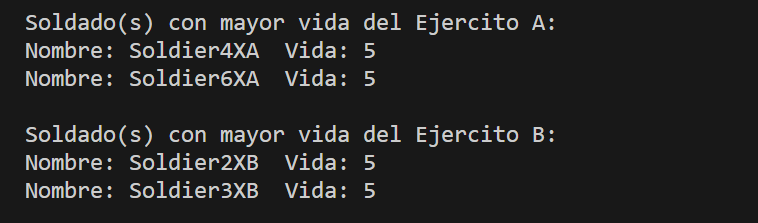
\includegraphics[width=0.7\textwidth,keepaspectratio]{img/moreHealth.png}
            \caption{}
        \end{figure}

        \begin{lstlisting}[language=bash,caption={Commit \href{https://github.com/hernanchoquehuanca/fp2-23b/commit/ba455c468a7dbaa2b26c2391aac7c93c0020d5f6}{ba455c4}: Se agregó el método moreHealt() que imprimirá aquellos soldados que tengan la mayor vida dentro de su ejército}][H]
    		$ git add .
    		$ git commit -m "Redefiniendo el metodo moreHealth, el cual mostrara aquellos soldados o soldado con mas vida dentro del ejercito que reciba como parametro"
    		$ git push -u origin main
    	\end{lstlisting}
        
        %%%%%%%%%%%%%%%%
        
        \subsubsection{Método para hallar la suma de vida en un ejército}

        \begin{itemize}
            \item El método tiene como nombre \textcolor{blue}{sumHealth()}.
            \item Se utiliza un entero inicializado en 0 para mientras que se recorre el ArrayList unidimensional de Soldado con un bucle for each, este entero (sum) va almacenando la vida de todos los soldados.
            \item Finalmente se retorna el entero \textcolor{blue}{sum}.
        \end{itemize}

        \lstinputlisting[language=Java, firstline=162, lastline=167,firstnumber=162,numbers=left]{src/VideoJuego4.java}
        \newpage
        \begin{itemize}
            \begin{itemize}
                \item Un ejemplo de como se muestra en la siguiente imagen:
            \end{itemize}
        \end{itemize}

        \begin{figure}[H]
            \centering
            
\includegraphics[width=0.7\textwidth,keepaspectratio]{img/sumHealth.png}
            \caption{}
        \end{figure}

        \begin{figure}[H]
            \centering
            
\includegraphics[width=0.7\textwidth,keepaspectratio]{img/sumHealth2.png}
            \caption{}
        \end{figure}
        
        %%%%%%%%%%%%%%%%
        
        \subsubsection{Método para hallar el promedio de vida en un ejército}

        \begin{itemize}
            \item El método tiene como nombre \textcolor{blue}{averageHealth()}.
            \item De manera breve como el método, este retorna una división entre la suma de la vida del ejército, haciendo uso del método \textcolor{blue}{sumHealth()} y dividiendo entre el tamaño del ejército.
        \end{itemize}

        \lstinputlisting[language=Java, firstline=158, lastline=160,firstnumber=158,numbers=left]{src/VideoJuego4.java}

        \begin{itemize}
            \begin{itemize}
                \item Un ejemplo de como se muestra en la siguiente imagen:
            \end{itemize}
        \end{itemize}

        \begin{figure}[H]
            \centering
            
\includegraphics[width=0.7\textwidth,keepaspectratio]{img/averageHealth.png}
            \caption{}
        \end{figure}

        \begin{figure}[H]
            \centering
            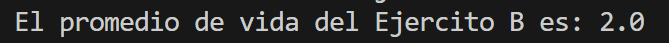
\includegraphics[width=0.7\textwidth,keepaspectratio]{img/averageHealth2.png}
            \caption{}
        \end{figure}

        \begin{lstlisting}[language=bash,caption={Commit \href{https://github.com/hernanchoquehuanca/fp2-23b/commit/422d59ae905d11466ef8011ef054ded358973c34}{422d59a}: Se agregó el método averageHealth y sumHealth, siendo el segundo de utilidad para el primero}][H]
    		$ git add .
    		$ git commit -m "Redefiniendo el metodo averageHealth, el cual calcula el promedio de vida de soldados en un ejercito, hace uso de un metodo llamado sumHealth que calcula la suma de la vida en un ejercito"
    		$ git push -u origin main
    	\end{lstlisting}
        
        %%%%%%%%%%%%%%%%
        \newpage
        \subsubsection{Método de ordenamiento BubbleSort}

        \begin{itemize}
            \item El método tiene como nombre \textcolor{blue}{bubbleSort()}.
            \item El método tiene como finalidad ordenar el ArrayList unidimensional de Soldado haciendo uso del algoritmo BubbleSort, tomando en cuenta la vida de los soldados que contiene cada soldado de dicho ArrayList. Este algoritmo se extrajo de Geeksforgeeks y fue adaptado a este proyecto. \textcolor{red}{Extraído tal cual del laboratorio anterior (lab06)}
        \end{itemize}

        \lstinputlisting[language=Java, firstline=169, lastline=186,firstnumber=169,numbers=left]{src/VideoJuego4.java}
        
        %%%%%%%%%%%%%%%%
        
        \subsubsection{Método de ordenamiento InsertionSort}
        
        \begin{itemize}
            \item El método tiene como nombre \textcolor{blue}{insertionSort()}.
            \item El método tiene como finalidad ordenar el ArrayList unidimensional de Soldado haciendo uso del algoritmo InsertionSort, tomando en cuenta la vida de los soldados que contiene cada soldado de dicho ArrayList. Este algoritmo se extrajo de Geeksforgeeks y fue adaptado a este proyecto. \textcolor{red}{Extraído tal cual del laboratorio anterior (lab06)}
        \end{itemize}
        
        \lstinputlisting[language=Java, firstline=188, lastline=203,firstnumber=188,numbers=left]{src/VideoJuego4.java}
        
        %%%%%%%%%%%%%%%%

        \subsubsection{Método de ordenamiento SelectionSort}

        \begin{itemize}
            \item El método tiene como nombre \textcolor{blue}{selectionSort()}.
            \item El método tiene como finalidad ordenar el ArrayList unidimensional de Soldado haciendo uso del algoritmo SelectionSort, tomando en cuenta la vida de los soldados que contiene cada soldado de dicho ArrayList. Este algoritmo se extrajo de Geeksforgeeks y fue adaptado a este proyecto. \textcolor{red}{Extraído tal cual del laboratorio anterior (lab06)}
        \end{itemize}

        \lstinputlisting[language=Java, firstline=205, lastline=221,firstnumber=205,numbers=left]{src/VideoJuego4.java}
        
        %%%%%%%%%%%%%%%%

        \subsubsection{Método para imprimir los soldados de un ejército, ordenados según su vida}
        
        \begin{itemize}
            \item El método tiene como nombre \textcolor{blue}{printArmyHealth()}.
            \item Este método recibirá un ArrayList unidimensional de Soldado (previamente ordenado), lo recorrerá usando un bucle for y mostrará los soldados, teniendo en cuenta que primero se mostrarán los de mayor vida hasta los de menor.
        \end{itemize}
        
        \lstinputlisting[language=Java, firstline=223, lastline=227,firstnumber=223,numbers=left]{src/VideoJuego4.java}

        \begin{lstlisting}[language=bash,caption={Commit \href{https://github.com/hernanchoquehuanca/fp2-23b/commit/fdb8f2cc3b507c74a19f0d255425c3a92b8a8206}{fdb8f2c}: Se implementaró el método printArmyHealth}][H]
    		$ git add .
    		$ git commit -m "Redefiniendo el metodo printArmyHealth, el cual nos muestra los ArrayList de ejercitos ya ordenados segun el nivel de vida (mayor a menor)"	
    		$ git push -u origin main
    	\end{lstlisting}
        \newpage
        \begin{itemize}
            \begin{itemize}
                \item Un ejemplo de como se muestra utilizando los 3 algoritmos de ordenamiento en la siguiente imagen:
            \end{itemize}
        \end{itemize}

        \begin{figure}[H]
            \centering
            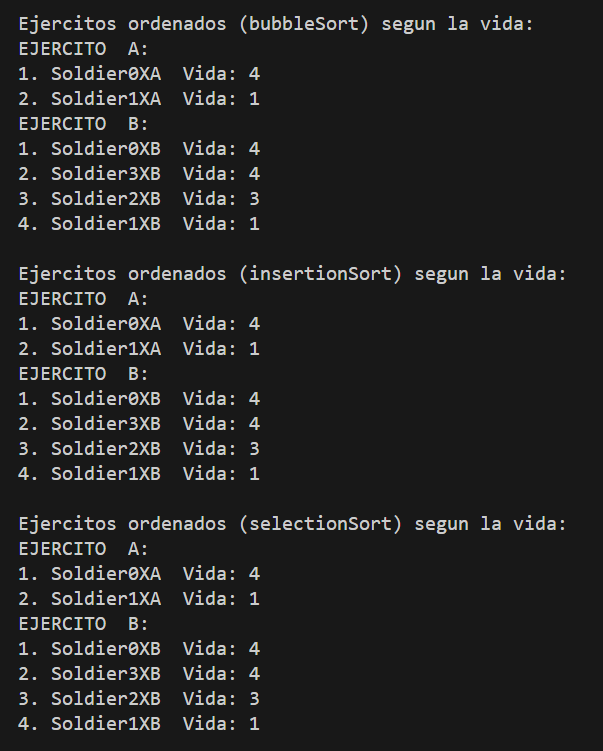
\includegraphics[width=0.6\textwidth,keepaspectratio]{img/printArmyHealth.png}
            \caption{}
        \end{figure}
        
        %%%%%%%%%%%%%%%%
        
        \subsubsection{Método para mostrar al ejército ganador según la vida de sus soldados}
        
        \begin{itemize}
            \item El método tiene como nombre \textcolor{blue}{armyWinnerHealth()}.
            \item Este método utilizará la suma de vida de cada ejército, hará comparaciones y si uno de los dos es superior en número de vida, se imprimirá que ganó, en caso de ser iguales mostrará aquello.
        \end{itemize}
        
        \lstinputlisting[language=Java, firstline=229, lastline=238,firstnumber=229,numbers=left]{src/VideoJuego4.java}

        \begin{lstlisting}[language=bash,caption={Commit \href{https://github.com/hernanchoquehuanca/fp2-23b/commit/e0d05ce1a7a50488f6f458c373a614a107d65489}{e0d05ce}: Se implementó el método armyWinnerHealth}][H]
    		$ git add .
    		$ git commit -m "Redefiniendo el metodo armyWinnerHealth, el cual muestra un ejercito ganador o empate dependiendo de la suma de vida de los ejercitos"	
    		$ git push -u origin main
    	\end{lstlisting}
        
        %%%%%%%%%%%%%%%%
        
        \subsubsection{Método para mostrar la interfaz y volver el programa iterativo}
        \begin{itemize}
            \item El método tiene como nombre \textcolor{blue}{mainInterfaz()}.
            \item Al iniciar esta pequeña interfaz, se muestra las acciones que se pueden realizar, las cuales se eligen escribiendo un número del 1 - 8 según se desee.
            \item Al terminar cada caso desde el 1 al 7, se vuelve a llamar al mismo método, esto lo vuelve iterativo.
            \item En el caso \textcolor{blue}{1}, se hace el llamado al método \textcolor{blue}{createArmy()}, esto para crear un nuevo ejército eliminando primero todos los ejércitos previamente creado (incluyendo el tablero).
            \item En el caso \textcolor{blue}{2}, se hace el llamado al método \textcolor{blue}{showArmyData()}, esto mostrará los soldados de ambos ejércitos (A - B) siguiendo el orden de su creación.
            \item En el caso \textcolor{blue}{3}, se hace el llamado al método \textcolor{blue}{showArmyTable()}, entonces mostrará el tablero con los soldados de ambos ejércitos, incluye su team, nombre y vida.
            \item En el caso \textcolor{blue}{4}, se hace el llamado al método \textcolor{blue}{averageHealth()}, será realizado para ambos ejércitos, mostrando así el promedio de vida en cada uno.
            \item En el caso \textcolor{blue}{5}, se hace el llamado al método \textcolor{blue}{moreHealth()}, aplicándolo a cada ejército mostrando así sus soldados con mayor cantidad de vida dentro de cada uno.
            \item En el caso \textcolor{blue}{6}, se hace el llamado al método \textcolor{blue}{printArmyHealth()}, dentro de este se llama a 3 métodos por cada ejército los cuales son algoritmos de ordenamiento que ordenarán sus soldados de mayor a menor vida, para luego mostrarlos en consola.
            \item En el caso \textcolor{blue}{7}, se hace el llamado al método \textcolor{blue}{armyWinnerHealth()}, mostrando así un ejército ganador en caso sus vidas no sean iguales, y en caso de que sí, mostrará aquello.
            \item En el caso \textcolor{blue}{8}, se muestra el mensaje \textcolor{violet}{Fin} ya que esta opción termina el programa.
            \item Y por último en caso de no ser ningún número anteriormente mencionado, se muestra un mensaje indicando que se debe seleccionar una opción válida, y se hace un llamado nuevamente a la función.
        \end{itemize}
\newpage
        \lstinputlisting[language=Java, firstline=16, lastline=86,firstnumber=16,numbers=left]{src/VideoJuego4.java}

        \begin{itemize}
            \begin{itemize}
                \item Un ejemplo de como se muestra en la siguiente imagen:
            \end{itemize}
        \end{itemize}
        
        \begin{figure}[H]
            \centering
            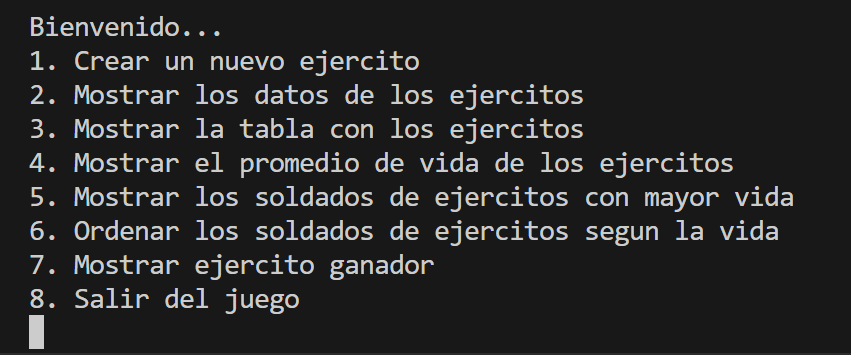
\includegraphics[width=0.8\textwidth,keepaspectratio]{img/mainInterfaz.png}
            \caption{}
        \end{figure}
    
        \begin{lstlisting}[language=bash,caption={Commit \href{https://github.com/hernanchoquehuanca/fp2-23b/commit/64fd210c75ca969277690eb4a062c3b393467098}{64fd210}: Se implementó el método mainInterfaz (PRIMER COMMIT)}][H]
    		$ git add .
    		$ git commit -m "Agregando el metodo interfaz, el cual sera utilizado para hacer nuestro programa iterativo"	
    		$ git push -u origin main
    	\end{lstlisting}

        \begin{lstlisting}[language=bash,caption={Commit \href{https://github.com/hernanchoquehuanca/fp2-23b/commit/390a95eba10e059c7a9662cba4fa90fcd0b0edf9}{390a95e}: Se implementó el switch dentro del método mainInterfaz (SEGUNDO COMMIT)}][H]
    		$ git add .
    		$ git commit -m "Implementando en el metodo mainInterfaz un switch para recibir la accion a realizar"	
    		$ git push -u origin main
    	\end{lstlisting}

        \begin{lstlisting}[language=bash,caption={Commit \href{https://github.com/hernanchoquehuanca/fp2-23b/commit/170f535a54c97bdb0ce65ff868320be5f5546e35}{170f535}: Se concluyó el switch dentro del método mainInterfaz tomando en cuenta todos los casos (ÚLTIMO COMMIT)}][H]
    		$ git add .
    		$ git commit -m "Implementando el caso 7 donde se muestra un ejercito ganador o empate, ya teniendo en cuenta la suma de vida de los soldados, esot dentro de la funcion mainInterfaz"	
    		$ git push -u origin main
    	\end{lstlisting}
        %%%%%%%%%%%%%%%%
        
        \subsubsection{Método main, utilización de los métodos creados}
        
        \begin{itemize}
            \item En el método principal (main) se utilizará simplemente dos métodos.
            \item Primero llamaremos al método \textcolor{blue}{createArmy()} que inicializará los ejércitos, quiere decir sus ArrayList y el tablero.
            \item Finalmente haciendo uso del método \textcolor{blue}{mainInterfaz()} se inicia el programa, ya que llamará a este y se ejecutarán los métodos según el usuario solicite y acabará hasta que este lo decida.
        \end{itemize}
        
        \lstinputlisting[language=Java, firstline=12, lastline=15,firstnumber=12,numbers=left]{src/VideoJuego4.java}
        
        %%%%%%%%%%%%%%%%
        
        \begin{lstlisting}[language=bash,caption={Commit \href{https://github.com/hernanchoquehuanca/fp2-23b/commit/5410f630dc5c356dbbbf0e370259d000622a6ea7}{5410f63}: Último commit, donde se implementó el método de la interfaz, sobre el cual está puesto los métodos del programa}][H]
    		$ git add .
    		$ git commit -m "Terminando el codigo, se adapto el interfaz al metodo main y se concluyo el metodo del mismo
    	\end{lstlisting}
     
%-----------------------------------------------------------------------------------
%------------------------------- DIAGRAMA DE CLASE ---------------------------------
%-----------------------------------------------------------------------------------
\newpage
        \subsection{Diagrama de clase UML}

        \begin{figure}[H]
            \centering
            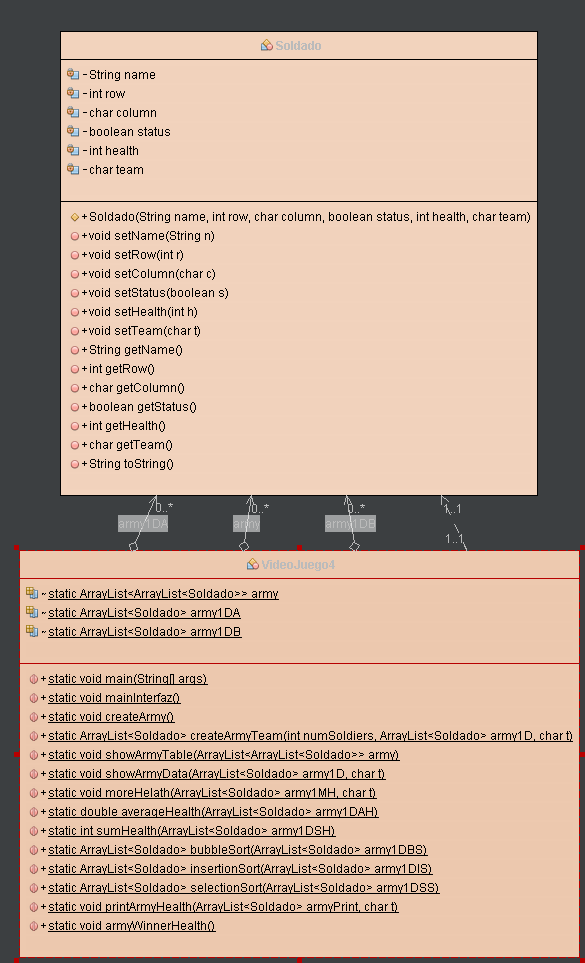
\includegraphics[width=0.75\textwidth,keepaspectratio]{img/diagrama07.png}
            \caption{}
        \end{figure}

%-----------------------------------------------------------------------------------
%------------------------------ ESTRUCTURA DE LABORATORIO --------------------------
%-----------------------------------------------------------------------------------
    \newpage
	\subsection{Estructura de laboratorio 07}
    \begin{itemize}	
		\item El contenido que se entrega en este laboratorio es el siguiente:
	\end{itemize}
	
\begin{lstlisting}[style=ascii-tree]

    lab07
    |   Soldado.java
    |   VideoJuego4.java
    |
    |───latex
        |   Informe_Lab07.pdf
        |   Informe_Lab07.tex
        |
        |───img
        |       averageHealth.png
        |       averageHealth2.png
        |       diagrama07.png
        |       logo_abet.png
        |       logo_episunsa.png
        |       logo_unsa.jpg
        |       mainInterfaz.png
        |       moreHealth.png
        |       printArmyHealth.png
        |       showArmyTable.png
        |       sumHealth.png
        |       sumHealth2.png
        |       toString.png
        |
        |───src
                Soldado.java
                VideoJuego4.java

\end{lstlisting}    

	\section{\textcolor{red}{Rúbricas}}
	
	\subsection{\textcolor{red}{Entregable Informe}}
	\begin{table}[H]
		\caption{Tipo de Informe}
		\setlength{\tabcolsep}{0.5em} % for the horizontal padding
		{\renewcommand{\arraystretch}{1.5} % for the vertical padding
		\begin{tabular}{|p{3cm}|p{12cm}|}
			\hline
			\multicolumn{2}{|c|}{\textbf{\textcolor{red}{Informe}}}  \\
			\hline 
			\textbf{\textcolor{red}{Latex}} & \textcolor{blue}{El informe está en formato PDF desde Latex,  con un formato limpio (buena presentación) y fácil de leer.}   \\ 
			\hline 
			
			
		\end{tabular}
	}
	\end{table}
	
	\clearpage
%-----------------------------------------------------------------------------------
%------------------------------ RÚBRICA DE EVALUACIÓN ------------------------------
%-----------------------------------------------------------------------------------
 
	\subsection{\textcolor{red}{Rúbrica para el contenido del Informe y demostración}}
	\begin{itemize}			
		\item El alumno debe marcar o dejar en blanco en celdas de la columna \textbf{Checklist} si cumplió con el ítem correspondiente.
		\item Si un alumno supera la fecha de entrega,  su calificación será sobre la nota mínima aprobada, siempre y cuando cumpla con todos lo ítems.
		\item El alumno debe auto calificarse en la columna \textbf{Estudiante} de acuerdo a la siguiente tabla:
	
		\begin{table}[ht]
			\caption{Niveles de desempeño}
			\begin{center}
			\begin{tabular}{ccccc}
    			\hline
    			 & \multicolumn{4}{c}{Nivel}\\
    			\cline{1-5}
    			\textbf{Puntos} & Insatisfactorio 25\%& En Proceso 50\% & Satisfactorio 75\% & Sobresaliente 100\%\\
    			\textbf{2.0}&0.5&1.0&1.5&2.0\\
    			\textbf{4.0}&1.0&2.0&3.0&4.0\\
    		\hline
			\end{tabular}
		\end{center}
	\end{table}	
	
	\end{itemize}
	
	\begin{table}[H]
		\caption{Rúbrica para contenido del Informe y demostración}
		\setlength{\tabcolsep}{0.5em} % for the horizontal padding
		{\renewcommand{\arraystretch}{1.5}% for the vertical padding
		%\begin{center}
		\begin{tabular}{|p{2.7cm}|p{7cm}|x{1.3cm}|p{1.2cm}|p{1.5cm}|p{1.1cm}|}
			\hline
    		\multicolumn{2}{|c|}{Contenido y demostración} & Puntos & Checklist & Estudiante & Profesor\\
			\hline
			\textbf{1. GitHub} & Hay enlace URL activo del directorio para el  laboratorio hacia su repositorio GitHub con código fuente terminado y fácil de revisar. &2 &X &2 & \\ 
			\hline
			\textbf{2. Commits} &  Hay capturas de pantalla de los commits más importantes con sus explicaciones detalladas. (El profesor puede preguntar para refrendar calificación). &4 &X &4 & \\ 
			\hline 
			\textbf{3. Código fuente} &  Hay porciones de código fuente importantes con numeración y explicaciones detalladas de sus funciones. &2 &X &2 & \\ 
			\hline 
			\textbf{4. Ejecución} & Se incluyen ejecuciones/pruebas del código fuente  explicadas gradualmente. &2 &X &2 & \\ 
			\hline			
			\textbf{5. Pregunta} & Se responde con completitud a la pregunta formulada en la tarea.  (El profesor puede preguntar para refrendar calificación).  &2 &X &2 & \\ 
			\hline	
			\textbf{6. Fechas} & Las fechas de modificación del código fuente están dentro de los plazos de fecha de entrega establecidos. &2 &X &2 & \\ 
			\hline 
			\textbf{7. Ortografía} & El documento no muestra errores ortográficos. &2 &X &2 & \\ 
			\hline 
			\textbf{8. Madurez} & El Informe muestra de manera general una evolución de la madurez del código fuente,  explicaciones puntuales pero precisas y un acabado impecable.   (El profesor puede preguntar para refrendar calificación).  &4 &X &3 & \\ 
			\hline
			\multicolumn{2}{|c|}{\textbf{Total}} &20 & &19 & \\ 
			\hline
		\end{tabular}
		%\end{center}
		%\label{tab:multicol}
		}
	\end{table}
	
\clearpage

%------------------------------ REFERENCIAS ------------------------------

\section{Referencias}
\begin{itemize}			
    \item \url{https://docs.oracle.com/javase/tutorial/java/nutsandbolts/variables.html}
    \item \url{https://docs.oracle.com/javase/8/docs/api/java/util/ArrayList.html}
    \item \url{https://docs.oracle.com/javase/tutorial/java/javaOO/methods.html}
    \item \url{https://www.geeksforgeeks.org/selection-sort/}
    \item \url{https://www.geeksforgeeks.org/bubble-sort/}
    \item \url{https://www.geeksforgeeks.org/insertion-sort/}
    \item \url{https://es.stackoverflow.com/questions/108171/}
\end{itemize}	
	
%\clearpage
%\bibliographystyle{apalike}
%\bibliographystyle{IEEEtranN}
%\bibliography{bibliography}
			
\end{document}